        % Chapter 1

\chapter{Summative Evaluation} % Main chapter title

\label{summativeevalchapter} % For referencing the chapter elsewhere, use \ref{Chapter1} 

\lhead{Chapter \ref{summativeevalchapter}. \emph{Summative Evaluation}} % This is for the header on each page - perhaps a shortened title

%----------------------------------------------------------------------------------------
\section{Recruitment of Participants}
With help of a research assistant who was a resident of Langa,  we managed to recruit a total of fourteen adult participants (beneficiary users) through a convenient sampling technique. Approaching of potential participants for recruitment was done in October 2015. We recruited these participants from two townships in Cape Town: Langa, and Athlone. In Langa there were five adult participants while in Athlone there were nine adult participants. The was only one male out of fourteen adult participants. Gender imbalance was as the result of females being more eager to participate than males. This trend of domination of females was also apparent in the study reported in Chapter \ref{prototype2chapter}. The average age of these adult participants was 44.21 years with a standard deviation (S.D) of 9.99 years and their age range of was between 26 and 60 years of age. The highest education level was secondary school and the lowest was the last grade of primary school. After recruitment of adults they were requested to elect one of their children/grand children to become their respective intermediary user; hence forming a pair of users. As the result fourteen children were recruited. Thirteen adult participants teamed up with their children, the remaining adult teamed up with her grand child. Children participants had a mean age of 15.42 (with a standard deviations of 2.06 years). The age range children participants was between 12  and 20 years of age. There was a gender balance on intermediary participants. 

I gave out detailed information of what the study was all about to both intermediary and beneficiary participants. I informed them about different modes of which I will be collecting data and these approaches included usage logs, questionnaires, and interviews. All the beneficiary participants signed informed consent forms agreeing to be part of the study. Since all intermediaries were under 21 years of age (legal age for giving consent in South Africa is 21 and above), they signed assent forms which were also signed by their respective parents/guardians who were part of the study.

One day was allocated for training intermediary participants on how to use the ``Family Wellness App''. In addition, each intermediary user was given a user manual. After the training, I gave out one Android phone (Samsung GT-S5300) to each pair of participants. These phones were installed with two natives apps. The first app was a pedometer and the second one was the main ``Family Wellness App''. The ``Family Wellness App'' loaded all its content from a web application hosted remotely from a server hosted at University of Cape Town. Each beneficiary participant was required to carry around the phone that was given to a pair in order for the pedometer app to count their footsteps. The two apps (main app and pedometer) were made available to the pairs of participants for a total period of six weeks. Each pair of participants provided the service provider's number of the SIM card that was inserted on their given Android phone. I allocated 1.3 GB of data to each SIM card. In addition each beneficiary participant was given a total of ZAR (South African Rands) 240 for the duration of the study. That amount of money covered for compensation for participants' transportation and time spent in data collection activities such as administering of questionnaires and interviews. The details of the experiments are outlined on the next section. 
\section{Experiments}
The main objective was to carry out experiments to evaluate the effectiveness of gamification in motivating  intermediated use. As the result, the experiments entailed comparisons between the app that was not gamified and the gamified app. The app that was not gamified was simply a diary that could enable individual pairs  to track diet/nutritional components of meals consumed by a beneficiary participant, ans secondly  to enable pairs to track footsteps walked by a beneficiary participant. The second version of the application was an extension of logbook meaning that it included all the features in logbook  with an addition of a rewards/gamified subsystem. The experiments took place from the mid-October 2015 to the end of November 2015.  The details of how experiments were designed and how data were collected are presented on the next sub-section.
\subsection{Experiment Design}
The study used ``within-group'' design for the experiments which used the same group of participants for both logbook and gamification. The rationale for this design was to reduce interference from confounding factors and in addition to reduce the cost of recruitment as the same group was for both control and intervention.he only problem with this approach is the learning effect and in addition, it lengthens the duration of a study. Pairs of participants were to two separate groups that started with and finished with opposite experimental conditions. These groups were referred to as experimental sequences. In the first experimental sequence there were pairs that started with logbook and later switched to gamification. In the second experimental sequence there were pairs that started with gamification and later they were switched to logbook. I used the following abbreviations ``LG'' and ``GL'' to refer to respective first and second experimental sequences. The rationale behind having two experimental sequences was to give equal chances to both experimental conditions to start at the beginning and if there is there was the learning effect on the outcome then it could have affected both experimental conditions equally. Therefore the learning effects from the two experimental conditions were expected to cancel each other.

A total of seven pairs of participants were assigned to the LG group while the remaining seven pairs were assigned to the GL group. Both groups spent the first four weeks in their respective first experimental conditions of which were logbook app for the LG group and gamified app for the GL group. After 27 days (four weeks) each group was switched to a different experimental condition; hence after the switching, the LG group started using the gamified app while the GL group started using the logbook app. The second phase of the experiment lasted for a total of 14 days (two weeks). 

The explanation of why four weeks in phase 1 and two weeks in phase 2 is as follows. Initially the plan was to have the time spent on each experimental condition, be in three(3) weeks intervals, but phase 1 had extended beyond its allocated block of three weeks up to the fourth week as pairs of participants were not available for midpoint assessments at the end of the third week. Therefore, I carried out the midpoint assessment at the end of the fourth week. After the aforementioned assessment, pairs that were in gamified app were switched to logbook app, and those that were in logbook app were switched to gamified app. It was not feasible to extend phase 2 to go up to four weeks as phase 1 due complexity that was going to be introduced as the result of rescheduling duration of experiments from six to eight weeks. Rescheduling was impossible because it was approaching December of where most people travel for holidays, therefore, gathering participants during that time may have been impractical. As the result this shortened the duration of phase 2 to two weeks. 
\subsection{Research Methods}
Data collection was carried out through a triangulation of application's usage logs, questionnaires, and interviews. In the next subsections, the details of each of the three approaches are provided. 
\subsubsection{Family Wellness App Logs}
Application's logs consisted of information such; when there were users' activities on the app, which pair was accessing the app at that time, and what functionality was being accessed by that pair. Logs were categorized to their respective experimental conditions. Usage was characterized by two dimensions; (1) the number of sessions of where the app had user's activity from a particular pair of users, and (2) the number of times certain features were accessed by a particular pair of users (impressions). A new session was defined as a period of detection of user's activity in an absence of any activity from this user/pair in the past one hour or more. Impressions was defined as the number of times in which a certain feature had been viewed by a pair. So if multiple clicks by one user/pair on one feature happened within an interval of less than one minute between two consecutive clicks on the same feature, such multiple consecutive clicks were grouped as a single impression. If clicks on the same feature differed by a minute or more then the current click was treated as a new impression while the previous click belongs to the previous impression. Therefore, if the time difference between clicks on the same feature is beyond one minute, then it was assumed that the user had gone away or move to a different feature and they are coming to this feature for another iteration of clicks on the feature as the previous iteration of clicks within that feature they are visiting had finished. The purpose of computing pair's total impressions on each feature was to understand where users of the app were likely to go among many options of gamification features. i.e. leaderboard (score board), score badge, botanical garden, and fish tank (fish aquarium). 
 
There were two major analyses conducted on usage logs. The first analysis was a comparison of number of sessions between gamified app and logbook in two steps. This particular analysis had two dimensions.  The first dimension entailed comparing the daily total number of sessions between the two experimental conditions for 41 days of experiments. This was a comparison between daily total sessions of all users in logbook app and daily total sessions of all users in gamified app. The second dimension entailed a pairwise comparison of users' sessions in between logbook and gamification conditions (repeated measures for usage during logbook and usage during gamification by the same pair of users). In order to ensure this comparison of usage doesn't get affected by the difference in experimental durations between phase 1 (period before switching of experimental conditions) and phase 2 (period after switching of experimental conditions), I opted to use a relative (normalized) number of sessions  as a unit of measurement. In this case I used the number of sessions per day since the number of sessions on a particular experimental condition was relative to the number of days on which a particular version of the app was made available to the pair of users -- duration of deployment. This duration of deployment differed between the two  experimental conditions from participants within the same experimental sequence. For pairs that were assigned to LG group four and two weeks were  spent in logbook  and gamification respectively while for pairs that were assigned to GL, four and two weeks were spent in gamification and logbook respectively. This implies if a pair that belongs to an experimental group (sequence), \emph{Z} spent an \emph{X} amount of days in an experimental condition \emph{Y} and had \emph{n} number of sessions, then their normalized number of sessions in experimental condition \emph{Y} will be \emph{\textbf{n}} sessions divide by \emph{\textbf{X}} days. So in order to make a comparison on repeated measures of usage (usage of individual pairs between logbook and gamification conditions) the hypothesis of interest was as follows :

\begin{enumerate}
\item{Hypothesis 1}
\begin{itemize}
\item{H\SB{0}}:There is no difference in normalized number of sessions between a logbook app and gamified app
\item{H\SB{A}}:There is a difference in normalized number of sessions between a logbook app and gamified app
\end{itemize}
\end{enumerate}

In the process of doing the aforementioned comparison, a decision was made to exclude four pairs in testing the aforementioned hypothesis. These were pairs that faced hurdles on utilizing the app as the result of technical glitches and this affected their ability to fully experience both experimental conditions. The excluded pairs are listed on Table \ref{table:usageproblems}.

\begin{table}[h!]
  \begin{center}
    \caption{Excluded pairs as the result of technical glitches}
    \label{table:usageproblems}
	\begin{tabular}{|l|l|l|p{6cm}|}
		\hline
		&Pair&Group&Problem\\
		\hline
		1&Pair-A&GL-sequence &App failed to load due to poor internet signal\\
		\hline
		2&Pair-B&GL-sequence&This pair didn't have data bundles due misallocation. \\
		\hline
		3&Pair-C & LG-sequence.& Their pedometer had never transmitted any throughout the duration of the study.\\
		\hline
		4&Pair-D & LG-sequence.& Pedometer worked for a while before it stopped transmission of data.\\
	\hline
	\end{tabular}
  \end{center}
\end{table}

For \textbf{Pair-A}, the app failed to load every time the intermediary user tried to use it. As the results the intermediary participant complained to the researcher that the app was being unstable. After a follow up it was observed that in the house where this particular pair lived in there was a poor Internet signal, hence the app was always failing to load most of the time and this frustrated the intermediary user. The second pair (\textbf{Pair-B}), data was allocated to the wrong phone number at the beginning of the experiments but they never reported on time. These two pairs (Pair-A and Pair-B) had the lowest usage days which were 2 and 3 days respectively of which usage happened only in gamification condition.

For the last two pairs (\textbf{Pairs-C} and \textbf{Pair-D}) on Table \ref{table:usageproblems}, pedometers had malfunctioned; this affected their ability to experience gamification as other pairs. The two pairs started to experience the technical glitches while still in logbook condition before being switched to gamification condition.

The second major analysis on usage logs examined the impact of gamification features on internalization. Perceived usefulness is a predictor of internalization. This analysis was done by contrasting how number of impressions on certain gamification features affected perceived usefulness. The term``impressions'' has already been defined above as pair's frequency in viewing a particular feature. The total number of impressions on each of gamification feature was calculated for the number of days in which pairs were assigned to gamification condition. In this analysis all fourteen pairs were considered including the four that had technical glitches. Since this comparison only involved one experimental condition; hence all features had equal chances of being accessed provided that the user/pair had managed to get into the app. Also some feedbacks were delivered through SMS meaning that all pairs had received such interactions regardless of whether the App was accessible or not; therefore, it is under the assumption that pairs that had received SMS feedback could be in position of judging the perceived usefulness of the app. In addition to that, intermediary users were frequently interacting to each other in face to face manner to talk about things in the app. Another assumption is that regardless of the app presence intermediary users would perceive helping their parents on app usage as something that as something that is meaningful. Hence if the user/pair had never viewed a particular gamification feature, they would still get zero as the number of impressions in that feature. The objective was to understand how gamification features affected internalization. On literature review section (Chapter \ref{literaturereview}), four types of internalization of behaviour regulation were highlighted. Therefore, this analysis also view internalization with respect to the four types of behaviour regulation. The questionnaires that were used to capture aspects of internalization (perceived usefulness) are mentioned on the next sub-section together with other sub-scales of intrinsic motivation.

\subsubsection{Questionnaires}\label{methodsquestionnaire}
The research team administered questionnaires at baseline, mid-line (during switching of experimental conditions), and end-line. These questionnaires targeted both intermediary and beneficiary participants. The list of questionnaires that are described below are attached at the Appendices \ref{AppendixC} and \ref{AppendixD}.
\begin{enumerate}
\item{\textbf{Intermediaries}}
Intermediaries had three questionnaires that were administered at baseline, midline, and endline.
 
\begin{itemize}
\item{\textbf{Baseline Questionnaire}}: Intermediaries participants' baseline questionnaire had three sections. The first section captured demographic information such as age, gender, and number services/apps used on cellphones.The second section included an IMI (Intrinsic Motivation Inventory) questionnaire  to assess participants' intrinsic motivation in using cellphones. The third section included an IMI questionnaire to assess participants' intrinsic motivation in helping their parents with cellphone based tasks. 

\item{\textbf{Midline Questionnaire}}: Intermediaries participants' midline questionnaire had only one section which included an IMI questionnaire  to assess participants' intrinsic motivation in using the family wellness app.

\item{\textbf{Endline Questionnaire}}: Intermediaries participants' endline questionnaire had only one section which included an IMI questionnaire  to assess participants' intrinsic motivation in using the family wellness app.
\end{itemize}

\item{\textbf{Beneficiaries}}

\begin{itemize}
\item{\textbf{Baseline Questionnaire}}: Beneficiary participants' baseline questionnaire had four sections. The first section included an IMI questionnaire  to assess participants' intrinsic motivation in using the family wellness app. The third section included an IMI questionnaire to assess participants' intrinsic motivation in self-monitoring of diet/nutrition. The fourth section included an IMI questionnaire to assess participants' intrinsic motivation in self-monitoring of physical activity.

\item{\textbf{Midline Questionnaire}}:Beneficiary participants' midline questionnaire had three sections. The first section included an IMI questionnaire  to assess participants' intrinsic motivation in using the family wellness app. The third section included an IMI questionnaire to assess participants' intrinsic motivation in self-monitoring of diet/nutrition.The fourth section included an IMI questionnaire to assess participants' intrinsic motivation in self-monitoring of physical activity.

\item{\textbf{Endline Questionnaire}}: Beneficiary participants' endline questionnaire had three sections. The first section included an IMI questionnaire  to assess participants' intrinsic motivation in using the family wellness app. The third section included an IMI questionnaire to assess participants' intrinsic motivation in self-monitoring of diet/nutrition.The fourth section included an IMI questionnaire to assess participants' intrinsic motivation in self-monitoring of physical activity.
\end{itemize}
\end{enumerate}

I developed the IMI questionnaires based on procedures specified by a website maintained by authors of ``Self-Determination Theory''\footnote{http://www.selfdeterminationtheory.org/intrinsic-motivation-inventory/} (Richard Ryan and Edward Deci\citep{deci1985intrinsic}). I pretested these questionnaires during the informative evaluation of prototype II in chapter \ref{prototype2chapter}. The most important sub-scales for the theoretical construct of this research were perceived competence and perceived autonomy which are part of the three basic psychological needs. The relatedness sub-scale is not yet validated but it was included in all questionnaires. Other sub-scales that were included all questionnaires or some of the questionnaires were perceived enjoyment, and perceived useful. Perceived enjoyment is the only direct measure of intrinsic motivation while perceived competence and perceived autonomy are predictors of intrinsic motivation. Self-Determination theory suggests that a behaviour can be started as externally motivated and if external motivators support the three basic psychological needs which are relatedness, competitiveness, and autonomy then a behaviour that was once externally motivated to people can be internalized and the same people will start to perform an activity just because the find it resonating with their core values and beliefs. Perceived useful is a predictor of internalization.

In addition to the aforementioned sub-scales, perceived efforts also appears in specific questionnaires (i.e self-monitoring of diet and activity, use of cellphone). This additional sub-scale was included as part of the package of IMI inventory questionnaire as it may be directly linked to the important sub-scales. However, its results were of less interest to the theoretical constructs of this research.
  
The overall IMI scores were computed by averaging the scores from each sub-scales. In each question from the IMI sub scales, respondents were supposed to rate there experience in a scale of 1 to 7 points which means that 1 implies the statement is "not true at all" and 7 means the statement is "very true".

There were two main objectives of using the IMI questionnaire. The first objective was to assess the ability of the two prototypes in supporting the participants with the three basic psychological needs. The difference in experimental durations was expected not to have any effect on motivations to use either of the two systems since both logbook and gamification were both present in both phases of experiments. Therefore, effects on motivations due to different durations were expected to cancel each other during analysis. I compared between the capability of the two prototypes in affording three basic psychological needs suggested by self-determination theory. In addition, I also included perceptions on enjoyment as it is a direct measure of intrinsic motivation. The corresponding scales from the IMI questionnaire were administered at midline and endline . Therefore, there were four main sub-scales that were considered and these were; perceived autonomy, perceived competence, perceived enjoyment, and perceived relatedness. There were also one additional supporting sub scale which was perceived useful of which its purpose was to extract pattern on internalization as far as gamification features are concerned.

The second objective of using IMI questionnaires was to assess motivations/self-determinations of beneficiaries in self-monitoring of diet and activity, and motivation/self-determination to use cellphone of both intermediaries and beneficiaries. These IMI questionnaires included perceptions of beneficiaries on enjoyment, competence, autonomy, relatedness, enjoyment, effort, and usefulness.

The hypotheses of interest to both intermediaries and beneficiaries on intrinsic motivation's sub-scales related to usage of the app in different experimental conditions were:

\begin{enumerate}
 \setcounter{enumi}{1}
\item{Hypothesis 2}
\begin{itemize}
\item{H\SB{0}}:There is no difference in scores of perceived competence in using the app between a logbook app and gamified app
\item{H\SB{A}}:There is a difference in scores of perceived competence in using the app between a logbook app and gamified app.
\end{itemize}
\item{Hypothesis 3}
\begin{itemize}
\item{H\SB{0}}:There is no difference in scores perceived autonomy in using the app between a logbook app and gamified app
\item{H\SB{A}}:There is a difference in scores of perceived autonomy in using the app between a logbook app and gamified app
\end{itemize}
\item{Hypothesis 4}
\begin{itemize}
\item{H\SB{0}}:There is no difference in scores of perceived relatedness in using the app between a logbook app and gamified app
\item{H\SB{A}}:There is a difference in scores of perceived relatedness in using the app between a logbook app and gamified app
\end{itemize}
\end{enumerate}

Each of the four aforementioned hypotheses was tested twice. The first test was to intermediary users' scores and the second on beneficiary users' scores. There were also hypotheses of interest for beneficiaries in self-monitoring of behaviours reported below:

\begin{enumerate}
 \setcounter{enumi}{4}
\item{Hypothesis 5}
\begin{itemize}
\item{H\SB{0}}:There is no difference in the overall self-determination to self-monitor diet of between a logbook app and gamified app
\item{H\SB{A}}:There is a difference in the overall self-determination to self-monitor diet of between a logbook app and gamified app
\end{itemize}
\item{Hypothesis 6}
\begin{itemize}
\item{H\SB{0}}:There is no difference in the overall self-determination to self-monitor activity of between a logbook app and gamified app
\item{H\SB{A}}:There is a difference in the overall self-determination to self-monitor activity of between a logbook app and gamified app
\end{itemize}
\end{enumerate}

In the comparison for self-monitoring of diet and activity, the first IMI comparison  entailed comparing the IMI score of each participant at baseline, midline, and endline regardless of an experimental condition. In the second comparison I compared scores at baseline, and at both logbook and gamification conditions. The IMI score was computed from the average of scores obtained from perceived competence sub-scale, perceived autonomy sub-scale, perceived relatedness sub-scale, perceived enjoyment sub-scale, perceived effort sub-scale, and perceived usefulness sub-scale. I  used one way ANOVA with repeated measures to test if there was a difference  between scores at: (1) baseline, midline, and endline, and (2)baseline, logbook and gamification. I used Mauchy's test\footnote{Read more on how Mauchy's test is used from http://www.statisticshell.com/docs/repeatedmeasures.pdf} to checked if different measuring points had the same covariance in each ANOVA test I carried out and this helped in deciding of whether to ``Sphericity Assumed'',``Greenhouse-Geisser'', or ``Huynh-Feldt'' of SPSS output.

Before each statistical test including for all of the aforementioned hypotheseses, samples were tested to find if they follow normal distribution ``\emph{Shapiro-Wilk Normality Test}''\footnote{http://sdittami.altervista.org/shapirotest/ShapiroTest.html}) was used to test for normal distribution. For the case of paired samples, the difference between repeated measures of each data point was used to test for normality. In case there was no normality, I would apply a log transformation on the original data, and repeat the normality test again. If normality is achieved I would proceed into using statistical tests that assume normality. For the case of two dependent samples a student t test with repeated measures was used. For the case three dependent samples, a one way ANOVA with repeated measures was used. In all cases of repeated measured, normality was achieved on the original data, as the result only statistical tests that assume a  normal distribution were used.  For the case of of independent samples, each sample was tested for normality. In the absence of a normal distribution in any of the two independent samples, a log transformation was applied in this context. There was a case of two independent samples where a log transformation couldn't result into any normal distribution, therefore, as the result, it was resorted to the use of Mann-Whitney U Test (a non-parametric test for independent samples) as will be reported on the findings. 
 
\subsubsection{Interviews}
I also conducted short unstructured interviews at midline and endline. I selected fewer intermediaries and beneficiaries for the interviews. Interviews responses were important in supplementing data collected through questionnaires and application's logs. All the names used to refer to either which participant excerpts came from or just a particular participant, are pseudonyms to protect confidentiality of participants. Some of the participants quotes that are presented in the findings have also appeared in a publication~\citep{katule2016family} of which I was the first author. 
\section{Findings}
There were four primary outcomes in analysing the findings and these are: (1)usage trend of the app; (2) user experience/intrinsic motivation  of both intermediaries and intermediaries in using the app; (3) intrinsic motivation of beneficiaries in self-monitoring of diet/nutrition; and (4) intrinsic motivation of beneficiaries in self-monitoring of physical activity. Some of these findings are also reported in paper by~\citep{katule2016family}. On reporting age of participants on interview's excerpts, the notation \emph{yrs} refers to years. 
\subsection{Findings on Application's Logs}
\label{usageoutcome}
\begin{figure}[htbp]
  \centering
    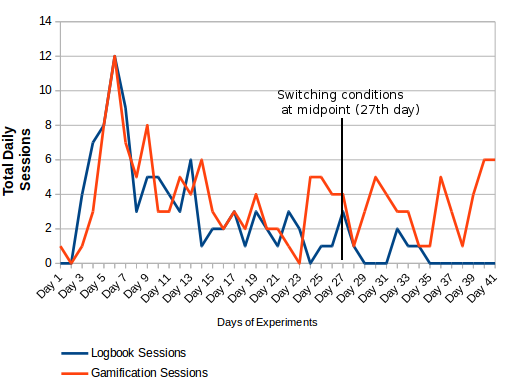
\includegraphics[width=0.6\textwidth]{Figures/scatter_daily_sessions.png}
    \rule{35em}{0.5pt}
  \caption{Total daily number of sessions from the two experimental conditions.}
  \label{figure:usagedailysessions}
\end{figure}
The average number of days on which pairs used both versions of the application was 10.5 (S.D = 7.39) days. The most active usage was from a pair that utilized the app for a total of 26 days. The less active usage was from a pair that had used the app for only two days out of 41 days. Figure \ref{figure:usagedailysessions} demonstrates trends on total daily usage's sessions in between logbook and gamification conditions. These trends indicate that in most days a gamified system had more total number of sessions compared to logbook. This is supported by a statistical comparison of daily total number sessions accumulated from all users in each experimental condition which showed that gamification condition had a significant total number of daily sessions compared to logbook as demonstrated by Mann-Whitney U Test on Table \ref{table:usagedays}.
\begin{table}[h!]
  \begin{center}
    \caption{Daily usage comparison between Logbook and Gamified systems for 41 days}
    \label{table:usagedays}
	\begin{tabular}{|L{3cm}|c|c|c|c|c|c|}
		\hline
		Groups&N (sample size)&Mean&Sum Ranks&U&Z&P\\
		\hline
   		Daily logbook sessions&41&33.72&1701.5&\multirow{2}{*}{1159.5}&\multirow{2}{*}{-2.9538}& \multirow{2}{*}{0.00318}\\\cline{1-4} 
   		 		    Daily gamification sessions&41&49.28& 1701.5&&&\\
\hline
	\end{tabular}
  \end{center}
\end{table}

\begin{figure}[htbp]
  \centering
    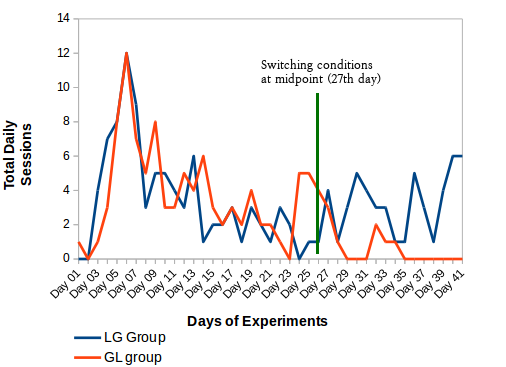
\includegraphics[width=0.6\textwidth]{Figures/usagedailysessions_lg_gl.png}
    \rule{35em}{0.5pt}
  \caption{Total daily number of sessions from the two experimental conditions.}
  \label{figure:usagedailysessions_lg_gl}
\end{figure}

An interesting phenomenon that expands on the usage pattern of Figure \ref{figure:usagedailysessions} above is that one of Figure \ref{figure:usagedailysessions_lg_gl} which shows usage trends of LG (logbook-gamification) and GL (gamification-logbook) groups. It can be observed that there is a sudden drop in number of usage sessions for users/pairs in GL group after being switched from gamification app to logbook app. This pattern suggests that most behaviour regulation during gamification condition was as the result of ego-involved (introjected regulation). This hypothesized situation is supported by a further exploration on number impressions on gamification features. On checking the average impressions among the four gamification, leaderboard seems to be having the highest average number of impressions as shown on Figure \ref{figure:gamification_impressions_latest_all}. 
\begin{figure}[htbp]
  \centering
    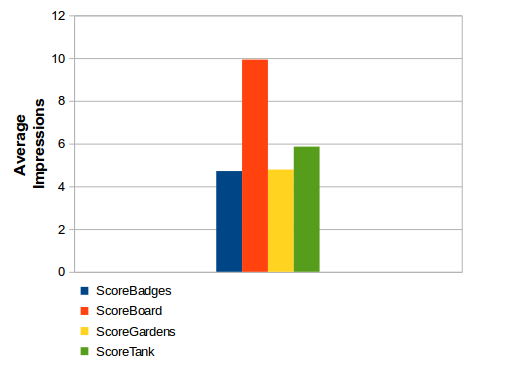
\includegraphics[width=0.6\textwidth]{Figures/gamification_impressions_latest_all.png}
    \rule{35em}{0.5pt}
  \caption{Total daily impressions for two groups (LG and GL).}
  \label{figure:gamification_impressions_latest_all}
\end{figure}
I conducted statistical comparison on the number of impressions between leaderboard and each of other gamification features (score badges, botanical garden, and fish tank). It was found that the number of impressions was statistically significant higher in leaderboard (Mean = 9.93;S.D = 13.90) compared to score badges (Mean =4.71, S.D = 5.50) (t (13) =2.1747, p = 0.0487). There was no statistical significance on either number of impressions between leaderboard (Mean = 9.93, S.D = 13.90) and botanical garden (Mean = 4.79, S.D = 5.26) (t(13)=1.716, p = 0.1096) or number of impressions between leaderboard (Mean = 9.93, S.D = 13.90) and fish tank (Mean = 5.86, S.D = 7.40) (t(13)=1.5707, p = 0.1403).However, the trend shows dominance of leaderboard over other gamification features. 

A further exploration on  gamification features' impressions revealed some insights on the trend of promotion of, ego involved, and task mastery, climates. This exploration follows the discussion of the previous chapter (Chapter \ref{prototype2chapter}) of where it was observed that some statements from qualitative feedback reflected that gamification features tended to promote either task mastery climate or ego-involved climate. In that previous discussion there was an inclination of the leaderboard to promote the ego-involved climate on some intermediary users while features like fish tank or botanical garden were inclined to promote the task mastery climate. Literature suggests that promotion of task mastery climate may foster integrated internalization of behaviour regulation while promotion of ego-involved climate may only promote introjected internalization of behaviour regulation~\citep{saksono2015spaceship}.

Since perceived usefulness is the only predictor of internalization as reported on the methods section above, therefore, one of the logical steps was to compare perceived usefulness scores between intermediary users who had visited leaderboard more often than other gamification features (number of impressions in leaderboard is greater than the number of impressions on any of the other gamification features) and those intermediary users whose number of impressions on leaderboard was almost similar or less to the number of impressions on any of the other gamification features. Since the average number of impressions on botanical garden, score badges, and fish tank were not so distant from each other as indicated on Figure \ref{figure:gamification_impressions_latest_all}, I selected only the botanical garden as a point reference (to represent features that may promote task master climate) for comparison with leaderboard(to represent those features that may promote ego-involved climate). Perceived usefulness was about how intermediaries rated the usefulness of the app to them and their parents. An assumption is that if the regulation is introjected then the intermediaries would careless about usefulness of the app. Therefore, the next task was to compare perceived usefulness between those intermediary users with high leaderboard impressions relative to the botanical garden and those with low leaderboard impressions relative to the botanical garden. In order to know whether an intermediary user falls under high or low group, the ratio was computed and this ratio was the number of impressions on leaderboard divide by the number of impressions on botanical garden. Two group were formed based on the median of ratios from all fourteen intermediary user which was 0.91. Seven intermediary users were assigned into a group with ratio~\textgreater=~\textbf{Median} while the remaining seven intermediary users where put under a group with ratio~\textless~\textbf{Median}. Therefore, the comparison was done on perceived usefulness of the gamified app between intermediary users with impressions' ratio~\textgreater=~\textbf{Median} and intermediary users with impressions' ratio~\textless~\textbf{Median}. The two independent samples followed a normal distribution; hence the results  of a student t test are shown on Table \ref{table:pu_leaderboard_bias}) which indicates that the group with ratio~\textless~\textbf{Median} scored significantly higher in perceived usefulness that the group with ratio~\textgreater=~\textbf{Median}. The implication of this finding is that those that had never accessed the leaderboard or had accessed it fewer times relative to the botanical garden had a higher tendency of valuing the intervention that utilized the gamified app as useful compared to those that had used the leaderboard relatively higher than the botanical garden. 

\begin{table}[h!]
  \begin{center}
    \caption{Comparison of perceived usefulness between group with ratio~\textgreater=~\textbf{Median} and group with ratio~\textless~\textbf{Median} (ratio = impressions on leaderboard/impressions on botanical garden)}
    \label{table:pu_leaderboard_bias}
	\begin{tabular}{|c|c|c|}
		\hline
		Mean &Group with ratio~\textgreater=~\textbf{Median}&Group with ratio~\textless~\textbf{Median}\\
		\hline
		 \multirow{2}{*}{Perceived usefulness}&Mean = 4.143 (S.D = 0.763)&Mean = 5.171 (S.D = 0.962)\\\cline{2-3} 

		 &\multicolumn{2}{|l|}{t(12) = 2.2156, p = 0.0468, 95\% CI = -2.040  to  -0.017} \\
\hline
	\end{tabular}
  \end{center}
\end{table}

Since the bias on usage of leaderboard showed the significant decrease of scores on perceived usefulness, the next task was to see if that affected gamification condition in general. Let's examine the trend of intermediaries' perceived usefulness between midpoint and endpoint between for both a group with ratio~\textgreater=~\textbf{Median} and ratio~\textless~\textbf{Median}. An earlier assumption was that the relationship between parents and children would make children to value the app as meaningful; hence the regulation would be considered as either identified or integrated regulation. But from the findings above, the trend indicated that most users concentrated on the leaderboard and as the result those with higher number of impressions of leaderboard compared to number of impressions on other gamification features such as the botanical garden appeared to have low scores in perceived usefulness. In order to verify the significance of the aforementioned trend,  the hypothesis of interest was that gamification affected the perceived usefulness of the app through its leaderboard feature. In order to prove this hypothesis, the logical step was to assess perceived usefulness between midpoint and endpoint for the two aforementioned groups. The perceived usefulness was statistically significant higher at endpoint (Mean = 5.4, S.D = 1.058) compared to midpoint (Mean = 4.67, S.D = 1.37) (t(6) = 4.9670, p = 0.0025) for the group with ratio~\textless~\textbf{Median} while for the group with ratio~\textgreater=~\textbf{Median}, there was no statistical significance difference between endpoint (Mean = 4.34, S.D = 1.081) and midpoint (Mean = 4.66, S.D =0.781) (t(6) = 0.8742, p =  0.4156). An intermediary user with the highest ratio, was the one with the lowest scores on perceived usefulness. There was a negative correlation between ratio of impressions (leaderboard/botanical garden) and perceived usefulness without statistical significance (r = 0.52, p = 0.06, N=14). What can be concluded so far is that it is very likely the leaderboard played a role in hindering internalization since perceived usefulness is a good predictor of internalization.  Also high usage of leaderboard suggests most usage in gamification was accounted as introjected regulation of where there is ego-involved. The presence of introjected regulation is supported by the excerpt below from one participant but it also emerges in most of the excerpts of users while in gamification condition. Therefore, usage in such cases is mostly influenced by the desire to dominate others in the competition.

\userquote{\textbf{Ayesha}, a beneficiary working with her son, 35 yrs} {``We [with Keagan] were not talking to others because all we wanted was to win. We didn't want them to know but they could see from the app''}

A different dimension of usage was the one that compares if there was a significance difference on number sessions between two experimental conditions (repeated measures of the same pairs at logbook and gamification conditions). As highlighted in the section that describes the methods above, the four pairs with technical glitches were excluded in order to bring fairness in the comparison of the two experimental conditions (Table \ref{table:usageproblems}). It was showed that the mean of logarithmic transformed data of normalized number of sessions between gamification and logbook were significant different (t(9)= -2.6593, p= 0.0261)~\citep{katule2016family}. This implies that the number of times the app was used per day during the gamified condition was significant higher compared to when pairs were in logbook condition. The log mean had to be used in this comparison because the test for normality on differences of data points between logbook and gamification failed. Therefore, a natural logarithmic transformation rectified the situation.

On the next sub sections, user experiences of both intermediaries and beneficiaries are reported.
\subsection{Intermediaries' User Experience}
In most cases, usage of the app within a pair of users was facilitated by intermediary users in proximate enabling and proximate translation. These types of intermediated interactions have been discussed in the work by \cite{sambasivan2010}. Baseline data indicated that interest of intermediary participants in using cellphones was higher than that beneficiary participants. For instance, in overall IMI scores to use cellphone, intermediaries (Mean = 5.76, S.D= 0.41, N=14) scored  significantly higher than beneficiary participants (Mean = 5.06, S.D= 0.71, N=13) with (t(25)= 3.1764, p = 0.0039, 95\% CI = 0.2472 to 1.1589).

If we refer back to the trend on Figure \ref{figure:usagedailysessions_lg_gl}, at the first days of experiments both gamification and logbook have patterns that are similar. However, after the second week logbook starts to go down on usage while the trend on gamification remained steady for a couple of days. One of the possible explanation of why logbook had the same effect as gamification at the beginning is because both experimental conditions had the novelty effect which was worn out after few days. Also the phone effect had contributed to high usage to most users in logbook condition during the phase 1 of experiments. The phenomenon of sharing intervention's phones was important in nurturing the relationship between intermediaries and beneficiaries. In cases where parents shared the intervention's phone with their respective children, children had a tendency to be more interested in the intervention. Children were using those phones for playing games and visiting online social networks. Therefore, free access to the intervention's phone played a role in increasing engagement of intermediary participants who didn't have their own smart-phones or data bundles in their smart-phones. In some cases, intermediary users installed other app on those phones such as games. To understand how the phone had a strong effect on motivation, the relationship between perceived autonomy to use cellphone at baseline and perceived enjoyment to use the app at midline was explored for the group that started with logbook. An interesting phenomenon was revealed. There was a significant negative relationship between perceived autonomy to use cellphone at baseline and perceived enjoyment to use the app at midline for the LG group (r=-0.84, p = 0.017, N=7). An explanation behind this is that those intermediary users with low autonomy to use cellphone had free access to the intervention  phone and this increased their interest to participate in the intervention. For instance one intermediary user (\textbf{Siphosethu}) from the LG group who was the youngest (12 years of age) among all reported the lowest score in perceived autonomy to use cellphone at baseline while reported the highest score in  perceived enjoyment to use the app at midpoint (after using logbook condition). She reported that she had freedom to use the intervention's phone

There was an inclination that a phone coupled with the novelty effect had mediated engagement for intermediaries that had started with the logbook condition. These intermediaries were helping their parents in return they got to have a free pass to access a cellphone. However, this finding is inconclusive due to the sample size. However, it highlights the discussion on the direction of what should be explored in future studies. For the GL group it was difficult to isolate the gamification effect from the phone and novelty affect and studies have shown that gamification has novelty effect, however, the trend shows that gamification accumulated more sessions compared to logbook hence gamification alone increased utilization of the family wellness app. Therefore, gamification appeared to be the most dominant factor that influenced usage as we have already seen that the frequency of usage showed a higher value in gamification when compared to logbook.

In additional to the novelty and phone effects, and gamification also another factor that contributed to intermediaries interaction with the family wellness app was requests from their respective beneficiaries.
There were times where intermediary users opened the app for interaction only upon receiving requests from beneficiaries. In both absence and presence of gamification, intermediaries had to fulfil requests from beneficiaries.  But during logbook condition, intermediaries appeared to be less enthusiastic in handling those requests. Some beneficiaries complained that there were several incidences of where their respective intermediary users were refusing to fulfil these requests and it happened more often during logbook condition. It was observed that in most of these cases, intermediary participants' autonomy was violated as requests came at times where intermediary participants were either studying for exams or doing something else and they felt it was not the right time to fulfil those requests. As the result, some of the intermediary participants to felt of being nagged by their parents. In one instance, a male intermediary participant appeared to be irritated by constant requests by his mother to interact with the app especially at the times when he is with he phone doing something else. Also a similar scenario was shared by one female intermediary participant who mentioned that her mother's constant demands to engage with the app were sometimes annoying as there was no excitement for her to the app as shown on the below excerpt.

\userquote{\textbf{Jennifer}, an intermediary for her mother, 18 yrs} {``The app was okay first but it started to get boring. You don't want to go into it any more. I think there will be some excitement now if the game comes in. When do we get the game''}

There were two motivational drivers for all requests that were put forward by beneficiary users. The first source of motivation was the instrumental value derived from using the app. The second reason is gamification. Requests that were mediated by gamification fostered a sense of collaboration between members of a pair while in the scenarios where beneficiaries were not concerned about gamification or during logbook conditions, requests tended to be of authoritative nature.

\userquote{\textbf{Ayesha}, a beneficiary working with her son , 35 yrs}{``I would always ask him [Keagan] where are we. Are we first? And what badge do we have? Where are the others? How far is Simon [intermediary] then? How far is that one? `No mum we are on top. We are first. We are the champions' [during gamification].''} 

The aforementioned excerpt from \textbf{Ayesha} demonstrates a sense of collaboration between the two members of a participating pair (\emph{Ayesha} and \emph{Keegan}). Therefore the presence of gamification in this context tended to promote a collective responsibility for pairs where both members of a pair were motivated by gamification unlike in logbook condition where there was an absence of that cooperation. The excerpt below came form a beneficiary participant in logbook condition and it indicated a beneficiary participant as having authority of what should be done and not a cooperation between members of a participating pair. 

\userquote{\textbf{Sisipho}, a beneficiary working with her son, 43 yrs} {``I always start the conversation. Because I always want to make sure if he records because I can't use it. It was difficult for me to use it. [during logbook]''}

The ``Gamified App'' was designed in such a way that a pair will earn rewards based on usage and the average number of steps walked by a beneficiary participant who is a member of the pair. The purpose of rewards was to foster users' intrinsic experiences such as competitiveness and a sense of autonomy which are predictors of intrinsic motivation with the goal of improving collaboration between members of a pair. Rewards depended on four parameters and these were the number of steps walked by a beneficiary user, the number of days the app has been used by an intermediary to either to record meals or to view feedback on meals, points, steps, gardens, etc. The presence of gamification nurtured  team work  even though the regulation of self-monitoring through intermediary users was mostly introjected (regulation done for the purpose of becoming better than others) as shown on below excerpts.

\userquote{\textbf{Keagan}, an intermediary for his mother, 16 yrs} {``When I see other people trying to come above me [on the leader board]. I hand over the phone to my mom so she can walk more steps.''}

\userquote{\textbf{Christine}, an intermediary for her mother, 16 yrs} {``I told my mom that me myself I want our team to have the highest points. Yes she said she is going to do that.''}

Through these collaborations goals were set of which in most cases they were set by intermediary users and informed their respective beneficiary about what they wish for the team (pair). A sense of joint ownership of the process was also common for these intermediary users as indicated by the following excerpts. 

\userquote{\textbf{Sophia}, an intermediary for her mother, 17 yrs} {``Sometimes that person may be first so I tell my mom that we must also be at the first place.[She looks at the  leader board and she sees other people at the first place, therefore, she talks to her mother that they should also aim for the first position] ''} 

\userquote{\textbf{Jenner}, a beneficiary working with her son, 45 yrs} {``When he [Leon] looked through it [The app] and sees their points, he would say `Mom, we need to do something here, because look at their points and our points'. So it was quite interesting.''} 

Comparison on virtual rewards among intermediary users motivated them to check the app more often compared to when they were in logbook condition as highlighted on the aforementioned usage findings (sub section \ref{usageoutcome}). Intermediaries were competing which each others through the leaderboard. As the result of this competition there were frequent face to face interactions that entailed comparing each other since most of them either attended the same schools or lived not far from each other. 

\userquote{\textbf{Jenner}, a beneficiary working with her son, 45 yrs} {``He [Leon (her 15 years old son) ] likes this exercise (using the app) because among him and his friends, they would have that competition like `I got more points than you' and that motivated him to get interested with the app''} 

Aforementioned cases above prove that regulation was mostly introjected as it was mediated by the need to be better than others in terms of points or being at the top of the leaderboard. Other features were not discussed in details in the interviews as intermediary users or beneficiary users who were interviewed didn't give any insights. The desire to be better mediated cheating the rules in some cases. For instance, there was a scenario of one pair of which not only the beneficiary user was using the pedometer, an intermediary was also taking turns to use the pedometer, therefore they were collaborating in accumulating steps. Both an intermediary user and a beneficiary user had discussions of whether the person whose turn it was had walk enough steps. They did this to accumulate more steps and hence more points than other pairs of users. 

\userquote{\textbf{Christine}, an intermediary for her mother, 16 yrs} {``I ask her how far did you walk?  She would say she walked very far. She tells me that I must have the phone to walk more steps. She would say `I got more more walking than you' [They were collaborating with her mother in accumulating steps]. She sometimes writes the steps on the page and she tells me yesterday I day I had more points than you [points referring to steps ]''} 

The ambiance of competition with others appeared to also affected pairs that had started with logbook conditions as some intermediary users were pushing their beneficiaries to do more by expecting to get rewards once they are switched to gamification condition; as the result during logbook condition there were intermediary participants who manifested ambitions to win while discussing with their respective beneficiaries~\citep{katule2016family}. The presence of gamification was also inclined to strengthen family bond or relatedness between members of a participating pair.

\userquote{\textbf{Khanyiswa}, a beneficiary working with her daughter, 26 years old} {``I think we talk more (with \textbf{Siphosethu}) than before the family wellness app. Before the family wellness app, after work it was just ``Hi'' and then I go to my room but now. But now she would come to my room  and say let me see your phone,  what did you eat today,  and write everything down on the phone.''} 

On the aspect of relatedness among intermediary users, social features were never utilized except by two users. One of those two users appeared to attempt to make a social connection with other users through the app. It was observed that this particular user was not collocated with other users; hence social features on the app was the only way to feel connected with others.  

\userquote{\textbf{Siphosethu}, an intermediary for her mother, 12 yrs } {``Wow it shows that you are working hard  Clara\#2.[She congratulated [Clara -a female aged 14 years old for having their fish tank ranked number 2 in quality.]''} 

The findings in user experience were mixed with some intermediary users having positive user experience on utilizing gamification while perceived enjoyment on some intermediary users was lower in gamification compared to logbook despite the fact that there were more sessions reported in gamification compared to logbook. Since the leaderboard drew most attention, it could have played a role in demotivating users with lower performance. Leader-board can demotivate those users that are at the bottom but it can foster aspects of relatedness for all users~\citep{sailer2013:psychological}. One way to exclude the impact of this on motivation was to single out intermediary users that never had any advancement in badges but had accessed to the leaderboard for at least two days or those intermediary users that never accessed any gamification feature due the app failing to load but seemed to be interested in accessing gamification features. I used badges as the point of measuring progress for those that had used the leaderboard for at least two days in a row or non consecutively. In this category there were two intermediary users that reported to have higher utilization of gamification features including the leaderboard and never made any progress in badges. These were among users that belonged to teams/pairs that were at the bottom of the leaderboard and their perceived enjoyment was lower in gamification condition compared to logbook condition.  One user was from the `LG' group (Keller), while the other one was from the `GL' group (Leon).  Their beneficiary participants were not walking enough steps despite the fact that these two intermediaries had put  more efforts in using the app during gamification condition than in logbook condition as shown on Figure \ref{figure:badge_failure_2}. 
\begin{figure}[htbp]
  \centering
    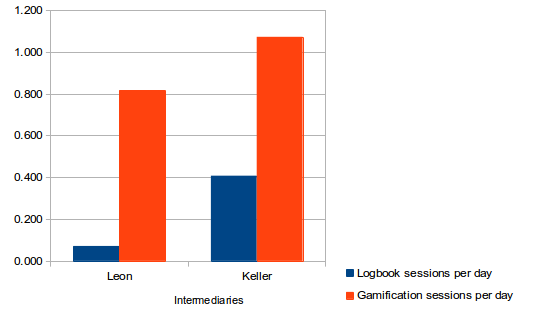
\includegraphics[width=0.7\textwidth]{Figures/badgesfailures2.png}
    \rule{35em}{0.5pt}
  \caption{Usage of two users without technical problems but lacked progress in badges.}
  \label{figure:badge_failure_2}
\end{figure} 

In the category of users with technical problems, there are two intermediary users of which one had attempted to access  the leaderboard and the pedometer was not working, and in the other user the app was failing to load completely hence couldn't access any feature. The two users in the latter category are part of the four users reported to be having usage problems as reported on Table \ref{table:usageproblems}. The remaining two users from Table \ref{table:usageproblems} never accessed a leaderboard although they had accessed other gamification features; hence were not so much exposed to the peer comparison as the result of using the leader-board although they had visited other gamification features. The perceived enjoyment of these two users who had accessed all gamification features except for the leaderboard was higher in gamification condition compared to logbook condition.    

There was also a case of where one user was a bit pessimistic about the credibility of the gamified system because her peers appeared to have more interest with the app, but were at lower positions on the leader board compared to her. 

\userquote{\textbf{Anathi}, an intermediary for her mother, 16 yrs} {``It [The experience in using the gamified app] was the same as last time (during logbook condition) except for the game part. I was actually above some of the others. That was weird. Because they were more interested in the app than me.[She was making a reference to intermediary users in pairs C and D that were found to experience technical problems as reported on Table \ref{table:usageproblems}]''} 

Anathi's anticipation was to see her peer being more competent than her once switched to gamification but contrary to her expectations she was ahead of them.  Therefore, this made her to doubt her competence. This further proved by her reported score on perceived competence between logbook and gamification. Anathi reported lower score in gamification compared to logbook despite using gamification for 7 out of 14 days and logbook for only 4 out of 27 days. However, Anathi had reported a slightly higher perceived enjoyment score  during gamification when compared to during logbook.

Therefore, in comparison between logbook and gamification for the support of the three basic psychological needs, a decision was made to exclude the four pairs whose perceived enjoyment was largely affected by either technical glitches or inability to participate fairly in gamification as the result of the app not being able to tailor challenges with skills of intermediary users as their performance relied to the great extent to the performance of their respective beneficiary users. For the intermediary users in the latter case, an assumption was that a negative experience was the result of failure of the gamification design to match challenges with abilities. i.e. efforts of beneficiary differed differed hence their performance had an effect on the overall performance of their respective team. This implies in that context, intermediary users had little control of the performance of their beneficiaries. Some intermediaries reacted in a negative way when they thought their respective intermediaries were not complying to carry the pedometer all the time.

\userquote{\textbf{Jenner}, a beneficiary working with her son, 45 yrs} {``Sometimes may be I forget to take the phone when I go walking and he would ask me `did you take the phone with you' Ooh Gosh I forgot.  Because when I walk to Park Town to exercise and sometimes  I am in such a hurry I forget the phone, he will be crossed with me.''} 

The aforementioned excerpt demonstrates how an intermediary user was attempting to control his beneficiary user as result competition influenced by peer pressure from intermediary users in other pairs. Therefore instead of gamification being something enjoyable in this context it resulted into a negative reaction that could threaten an existing social rapport between a parent and a child.

As for reasons stated above, four intermediary users in total were excluded in the analysis of self-determination theory. As the result only 10 out of 14 intermediary users were considered in the sub-scales that measured the three aspects of SDT (autonomy, competence, relatedness). On perceived competence to engage with the app, the gamified condition scored statistically significant higher than the logbook condition (t(9)=3.495, p = 0.0068)~\citep{katule2016family}. There was no significant difference between logbook and gamification on scores of perceived autonomy (t(9)= -0.027, p =  0.98) and perceived relatedness (t(9)= -0.719, p = 0.49)~\citep{katule2016family}.

\subsection{User Experience of Beneficiaries}
As most beneficiaries only interfaced with the app through intermediary users, beneficiaries' user experience relied on cooperation they got from intermediaries. On support for the three basic psychological needs, there was no difference between logbook and gamification. However, aspects of relatedness (N=14) appeared to improve significantly with time when in comparison between midpoint (Mean = 4.43, S.D=0.92) and endpoint (Mean = 5.38, S.D=1.08)(t(13)= 2.3736, p =  0.0337). Therefore, the intervention in general made beneficiaries felt more related to others (their respective intermediaries and other beneficiaries) who were part of the intervention.
  
On utilizing the app through intermediaries, there are cases where beneficiaries had a negative experience as result of intermediaries refusing to assist upon being given requests. This happened in cases of where intermediary users didn't feel like helping because of being occupies by other tasks such as reading for exams or because they felt the app was boring especially in logbook condition. 

In the next sub-section, the IMIs in self-monitoring of diet and activity are reported. Four pairs with usage problems (Table \ref{table:usageproblems}) were excluded due to their usage in self-monitoring being affected. Therefore, in total only ten out of fourteen beneficiaries had their results included for analysis in order to have only beneficiaries who had meaningful engagement with the app through their respective intermediaries.
\subsubsection{IMI in Self-Monitoring of Diet}
The results on self-monitoring of diet (baseline, midline, and endline) are shown on Table  \ref{table:imidietbenf}. The Mauchly’s test indicated that the assumption of sphericity was not violated with  $\chi{}$\SP{2}(2)=3.76, p = 0.152. The results (N=10) on  ``Self-monitoring of Diet'' shown on Table \ref{table:imidietbenf} were from ``Sphericity Assumed'' output. ANOVA showed that there was a significant difference of average IMI scores on self-monitoring of diet measured at baseline, midline and endline.
\begin{table}[h!]
  \begin{center}
    \caption{Comparison of ten beneficiaries' IMI scores in self-monitoring of diet at baseline, midline and endline}
    \label{table:imidietbenf}
	\begin{tabular}{|L{2.8cm}|L{3.2cm}|L{3.2cm}|L{3.2cm}|}
		\hline
		Mean IMI Score &Baseline&Midline&Endline\\
		\hline
		 %\multirow{3}{*}
		 {Self-monitoring}&Mean = 4.48; S.D = 1.24&Mean = 5.07; S.D = 1.19;&Mean = 5.55; S.D = 0.95\\\cline{2-4} 

		of Diet &\multicolumn{3}{|l|}{F(2,18)=3.787; p = 0.042} \\
\hline	\end{tabular}
  \end{center}
\end{table}
A finding from a pairwise comparisons (a paired student t-test) indicated that the IMI score at endline was significantly higher than at baseline (Table \ref{table:imipairwisediet}). There was no significant difference on baseline versus midline and midline versus endline (Tables \ref{table:imipairwisediet1}, and \ref{table:imipairwisediet2}). Motivation to self-monitor diet appeared to increase with time as shown on Figure \ref{figure:imi_diet}. The interpretation of the above findings are that the wellness app appeared to had a significant effect of time on motivation of beneficiaries to self-monitor their diet.
\begin{table}[h!]
  \begin{center}
    \caption{Pairwise comparisons of IMI scores in self-monitoring of diet: Baseline versus Midline}
    \label{table:imipairwisediet}
	\begin{tabular}{|L{2cm}|L{4cm}|L{4cm}|}
		\hline
		Mean &Baseline&Midline\\
		\hline
		 \multirow{2}{*}{IMI Score}&Mean = 4.48; S.D = 1.24&Mean = 5.07; S.D = 1.19\\\cline{2-3} 

		 &\multicolumn{2}{|l|}{t(9) = 1.298, p = 0.227} \\
\hline
	\end{tabular}
  \end{center}
\end{table}
\begin{table}[h!]
  \begin{center}
    \caption{Pairwise comparisons of IMI scores in self-monitoring of diet: Baseline versus Endline}
    \label{table:imipairwisediet1}
	\begin{tabular}{|L{2cm}|L{4cm}|L{4cm}|}
		\hline
		Mean &Baseline&Endline\\
		\hline
		 \multirow{2}{*}{IMI Score}&Mean = 4.48; S.D = 1.24&Mean = 5.55; S.D = 0.95\\\cline{2-3} 

		 &\multicolumn{2}{|l|}{t(9)= 2.457, p = 0.036} \\
\hline
	\end{tabular}
  \end{center}
\end{table}
\begin{table}[h!]
  \begin{center}
    \caption{Pairwise comparisons of IMI scores in self-monitoring of diet: Midline versus Endline}
    \label{table:imipairwisediet2}
	\begin{tabular}{|L{2cm}|L{4cm}|L{4cm}|}
		\hline
		Mean &Midline&Endline\\
		\hline
		 \multirow{2}{*}{IMI Score}&Mean = 5.07; S.D = 1.19&Mean = 5.55; S.D = 0.95\\\cline{2-3} 

		 &\multicolumn{2}{|l|}{t(9)=-1.975; p = 0.08 ; 95\% CI= -1.0342 to 0.07017} \\
\hline
	\end{tabular}
  \end{center}
\end{table}

\begin{figure}[htbp]
  \centering
    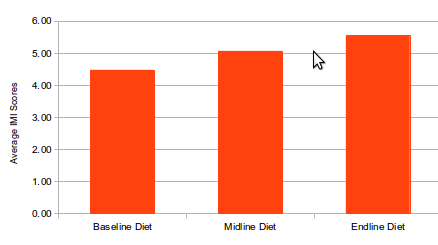
\includegraphics[width=0.4\textwidth]{Figures/imi_diet.png}
    \rule{35em}{0.5pt}
  \caption{Trend on Average IMI Scores of Self-Monitoring of Diet at Baseline, Midline, and Endline.}
  \label{figure:imi_diet}
\end{figure}
The aforementioned ANOVA finding on comparison among baseline, midline, and endline doesn't discern between different experimental conditions of which pairs of users were exposed to. The ANOVA finding (N=10)(Table  \ref{table:imidietbenf2}) on the comparison of IMI scores to self-monitor diet, among baseline, logbook, and gamification conditions showed that there was no significant difference of average IMI scores on self-monitoring of diet measured during baseline, logbook and gamification conditions. This finding is from the ``Sphericity Assumed'' output of the ANOVA test since the Mauchly’s test indicated that the assumption of sphericity was not violated with  $\chi{}$\SP{2}(2)=2.19, p = 0.335. The trend on averages shows both logbook and gamification to be slightly higher than baseline as shown on Figure \ref{figure:imi_diet2}. The conclusion from this finding is that both versions of the prototype have shown an indication of increasing motivation of beneficiaries to self-monitor diet.
\begin{table}[h!]
  \begin{center}
    \caption{Comparison of ten beneficiaries' IMI scores in self-monitoring of diet at baseline, after logbook, and  after gamification conditions}
    \label{table:imidietbenf2}
	\begin{tabular}{|L{2.8cm}|L{2.5cm}|L{2.5cm}|L{2.5cm}|}
		\hline
		Mean IMI Score &Baseline&Logbook&Gamification\\
		\hline
		 %\multirow{3}{*}
		 Self-monitoring&Mean = 4.48; S.D = 1.241&Mean = 5.28; S.D = 1.05&Mean = 5.34; S.D = 1.16\\\cline{2-4} 
		 of Diet&\multicolumn{3}{|l|}{F(2,18)=3.787; p = 0.087} \\
\hline	\end{tabular}
  \end{center}
\end{table}
\begin{figure}[htbp]
  \centering
    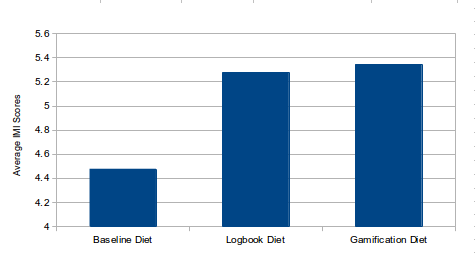
\includegraphics[width=0.4\textwidth]{Figures/imi_diet2.png}
    \rule{35em}{0.5pt}
  \caption{Trend on Average IMI Scores of Self-Monitoring of Diet at Baseline, Logbook, and Gamification.}
  \label{figure:imi_diet2}
\end{figure}
\subsubsection{IMI in Self-Monitoring of Activity}
The results (N=9) on self-monitoring of activity are shown on Table  \ref{table:imiactivitybenf}. The results are based on a sample of nine beneficiary users as one participant didn't complete this part of the questionnaire at baseline.  The Mauchly’s test indicated that the assumption of sphericity was violated with  $\chi{}$\SP{2}(2)=8.248, p = 0.016. The value $\epsilon$ on Greenhouse Geisser was ``\textless 0.75'', therefore, the results on  ``Self-monitoring of Diet'' shown on Table \ref{table:imiactivitybenf} were selected from ``Greenhouse-Geisser'' output. ANOVA showed that there was no significant difference of average IMI scores on self-monitoring of activity measured at baseline, midline and endline. The trend of means appears to increase from baseline to endline as shown on Figure \ref{figure:imi_activity}.

There are several factors that could have contributed to results not being significant among baseline, midline,endline points,. The first hypothesized reason is tracking of physical activity appeared to be easy in majority of the participants even without tracking devices as people can estimate the distance they walk daily and they consider this as tracking even though they might have means to record this information, hence their motivation was high at baseline unlike diet self-monitoring which they consider it to be cumbersome due to external barriers such as health food being expensive, therefore at baseline participants felt more motivated to track their activity. The second hypothesized reason is that the sample size was small hence there was a smaller power in detecting significant difference. But we have seen that the trend in motivation increases with time.
\begin{table}[h!]
  \begin{center}
    \caption{Comparison of ten beneficiaries' IMI scores in self-monitoring of activity at baseline, midline and endline}
    \label{table:imiactivitybenf}
	\begin{tabular}{|L{2.8cm}|L{2.5cm}|L{2.5cm}|L{2.5cm}|}
		\hline
		Mean IMI Score &Baseline&Midline&Endline\\
		\hline
		 %\multirow{3}{*}
		 Self-monitoring&Mean = 4.82; S.D = 1.002&Mean = 5.28; S.D = 1.003&Mean = 5.41; S.D = 0.894\\\cline{2-4} 
		 of activity&\multicolumn{3}{|l|}{F(1.182, 9.455)=2.936; p = 0.116} \\
\hline	\end{tabular}
  \end{center}
\end{table}

\begin{figure}[htbp]
  \centering
    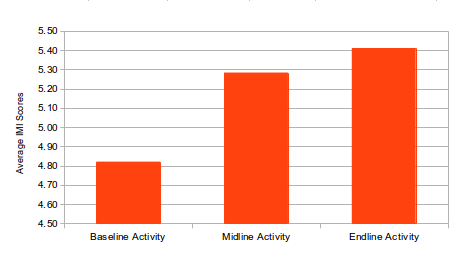
\includegraphics[width=0.4\textwidth]{Figures/imi_activity.png}
    \rule{35em}{0.5pt}
  \caption{Trend on Average IMI Scores of Self-Monitoring of Activity at Baseline, Logbook, and Gamification.}
  \label{figure:imi_activity}
\end{figure}
The finding from an analysis (N=9) that examined if there is a difference among baseline,logbook, and gamification in self-monitoring of activity, showed that there was no significant difference of average IMI scores on self-monitoring of activity measured at baseline, logbook and gamification (Table {table:imiactivity2benf}). The Mauchly’s test indicated that the assumption of sphericity was violated with  $\chi{}$\SP{2}(2)=6.788, p =0.034. The value of $\epsilon$ on Greenhouse Geisser was ``\textless 0.75'', therefore, these results on  ``Self-monitoring of Activity'' were selected from ``Greenhouse-Geisser'' output of oen way with repeated measures ANOVA test. The trend in motivation increases in both logbook and gamification compared to baseline as shown on Figure \ref{figure:imi_activity2}
%epsilon=0.617
\begin{table}[h!]
  \begin{center}
    \caption{Comparison of ten beneficiaries' IMI scores in self-monitoring of activity at baseline, logbook and gamification}
    \label{table:imiactivity2benf}
	\begin{tabular}{|L{2.8cm}|L{2.5cm}|L{2.5cm}|L{2.5cm}|}
		\hline
		Mean IMI Score &Baseline&Logbook&Gamification\\
		\hline
		 %\multirow{3}{*}
		 Self-monitoring&Mean = 4.82; S.D = 1.002&Mean = 5.33; S.D = 0.9762&Mean = 5.37; S.D = 0.9276\\\cline{2-4} 
		 of activity&\multicolumn{3}{|l|}{F(1.234, 9.872)=2.783; p = 0.123} \\
\hline	\end{tabular}
  \end{center}
\end{table}
\begin{figure}[htbp]
  \centering
    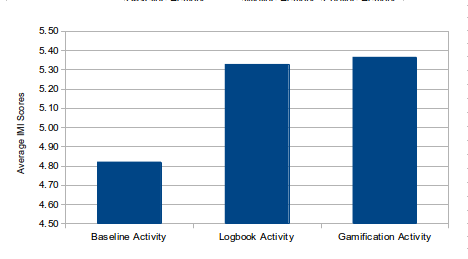
\includegraphics[width=0.4\textwidth]{Figures/imi_activity2.png}
    \rule{35em}{0.5pt}
  \caption{Trend on Average IMI Scores of Self-Monitoring of Activity at Baseline, Logbook, and Gamification.}
  \label{figure:imi_activity2}
\end{figure}

\section{Discussion}
\subsection{Motivational Affordances' Impact on Intermediaries}
As reported above intermediary users facilitated interaction with the app. Intermediaries were motivated to engage with the app mostly because of two main reasons and these were: either to follow up on competition with others or to serve requests from their respective beneficiary users. Gamification was the main source of motivation to intermediaries and it played a pivotal role in mediating usage during gamification condition or even in logbook condition for intermediary users in pairs that had started with logbook condition before being switched to gamification condition. Expectation of gamification condition at a later stage by some users who had started with logbook condition motivated them to sustain engagement while in logbook before being switched to condition. For instance in a case of \textbf{Siphosethu}, an intermediary user who talked of winning while still in logbook condition. Therefore, this affected the separation of experimental conditions since the randomization to experimental sequences was not blind; hence those that started with logbook already knew that they will start using gamification after a period of three weeks and this positively affected their behaviour towards engagement with the app. On perceived competence, the difference between logbook and gamification was statistically significant meaning intermediary users in gamification felt more competent.Statistical significance in difference was not achieved in cases of autonomy and relatedness due to the learning effect and a smaller sample size.  Perceived competence and perceived autonomy are the most important predictors of intrinsic motivation. 

From the findings it is also evident that gamification played a role in improving intermediaries' perceived enjoyment (a direct measure of intrinsic motivation) in using the app except for fewer cases of where it appeared to harm  perceived enjoyment due to several reasons that have already been highlighted on the findings section above. For instance the use of leaderboard contributed to both positive and negative depending on individual characteristics of an intermediary user and characteristics of a team in general. Intermediary users responded differently to gamification due to a great variation in users' traits (personalities) and skills possessed by their respective team mates (beneficiaries) of where this contributed to having such mixed results. Literature has vastly explored how important it is to tailor game design mechanics to players' personalities. In one survey that investigated how preferences of motivational affordances is linked to individuals' personality traits concluded with some of the following insights: (1) extraverts tend to be motivated by points, levels, and leaderboard; (2) avatars are likely to be preferred by people with high levels imagination; (3) extraverts prefer to be centre of the stage; hence the position they desire in a feature like a leaderboard is the top one; (4) introverts may not be happy to be in a crowd of strangers; (5) and so on..~\citep{jia2016personality}. Personalities that are exhibited by game players may also cross to gamification since the boundary between gamification and games is diminishing~\citep{ferro2013towards}. What may be considered just as a simple gamified system in one context may be socially perceived as a game in a different context~\citep{deterding2011game}. Personalization of healthy interventions to gamer types  is already common\cite{arteaga2010:persuasive,orji2013:tailoring} but has only been used in the context of direct users of technology and not in the context of intermediary and beneficiary users.

Apart from tailoring of game mechanics another aspect of personalization is on involuntary participation in gamification features. This brings to the subject of supporting autonomy. Gamification borrows its game mechanics from games and playing games has been pointed out as voluntary~\citep{seaborn2015:gamification,knaving2013designing}. Participating in a gamification layer should be an opt-in (invisible) and not a mandatory in order not to obscure the main activity being promoted~\citep{knaving2013designing}. In most of current gamification designs the line between voluntary and involuntary participation is not clear as a user may voluntarily participate in gamification but may not involuntarily participate in a feature like a leaderboard which may come as part of the package of gamification~\citep{ferro2013towards}. This brings to the subject of autonomy to users in selecting which of part of gamification features they would like to participate in. In addition to that, there is a different aspect of autonomy that was a shortcoming in this intervention and this is the inability of intermediary users to select the level of gamification appropriate to their skills. The only support for autonomy that was provided is the one that allowed configuration of avatars and editing of team profiles. Intermediaries stated goals as indicated in the findings but never had enough power in accomplishing those goals as the goals largely depended on skills possessed by their respective beneficiaries. Literature suggests approaches on which autonomy could be supported which include but not limited to configuration of profiles, avatars, macros, configurable interface, alternative activities, privacy control, etc. \citep{francisco2012analysis}. These approaches may scale to the context of technology use through intermediaries but there is a need to explore how intermediary users may have autonomy in formulation and execution of goals to tackle challenges based on their skills. When challenges are too difficult as they don't match users' skills, end users can become demotivated \citep{zhang2008motivational}.    

Absence of autonomy in formulation and execution of goals may foster  negative experiences which appeared to harm intrinsic motivation of some intermediary users in this context. For instance in most cases presence of gamification fostered collaboration between intermediary and beneficiary members of a pair. Out of this collaboration intermediaries were attempting to influence or persuade their respective beneficiaries. In such attempts negative experiences emanated when persuasion was not working. An example of a negative experience is the case of where nudging evolved into nagging like in a scenario we have seen above of \textbf{Jenner}, a beneficiary user who described how serious her son was taking the competition with others by constantly reminding her to carry the pedometer whenever she wants to go out and at times the son would get annoyed if his mother forgets to carry the pedometer. The ramification of this is that it deviates from the goal of promoting collaboration between an intermediary user and a beneficiary user and instead it creates a tension between them.  
In such scenarios intermediary users may react out frustration of not having control of the skills possessed by their respective beneficiaries; hence this idea of intermediaries to rely solely on skills of their respective beneficiaries seemed not to resonate with the notion of matching challenges to skills of users and it was the main source of tension between members of a pair as highlighted above. 

One of the approaches that could be used to minimize the effect of the  aforementioned shortcomings is to give users more autonomy to select different levels of gamification they want to participate. There could be levels such as beginners, intermediate, advanced, etc. Pairs that are on the same level could be grouped together and not mixed with pairs with levels that are different. In addition, users could be allowed to select which features they would like to include in their interfaces from a range of features such as chat rooms, leader-boards, botanical gardens etc. More autonomy can also be given in customization of privacy in terms of whether they would like to share their information or not. Customization of avatars is also important because It was observed that most users changed their avatars during gamification and one user explained that she sees the avatar she selected as a representation of herself. Through avatars, these users embodied their identities.

The second possible approach in increasing engagement of intermediary users is to allow intermediary participants to participate with their information, by incorporating their wellness data i.e. steps. The former can also be combined with the latter. There were some observed scenarios that support the utilization of the latter approach. For instance, there was one pair of whereby not only the beneficiary participant was using the pedometer as an intermediary was also using it. They were taking turns to use the pedometer, therefore, they were collaborating in accumulating steps. This pair had discussions of whether the person whose turn it was had walked enough steps. The goal was to accumulate more steps than other pairs. A similar concept has been explored with participants in a low income neighbourhood in USA , of whereby there is an exergame that encourages cooperation between parents and children~\citep{saksono2015spaceship}.

A third proposed way of increasing engagement that could be leveraged is the one reflected by intermediaries who claimed to also be benefiting from nutrition/diet information since the same type of meal is shared at home, therefore, if beneficiary participants ate something that is not healthy while at home then there is a likelihood of an intermediary participant to have eaten the same type of meal too. According to literature, parents who live a healthily lifestyle are likely to also influence their children to live healthily~\citep{grimes2009toward}. It is possible that by creating a system that allows intermediaries to also benefit from usage one can foster regulation that is either type \emph{identified} or type \emph{integrated} which are both on the side of the spectrum nearer to intrinsic motivation. 

Apart from gamification, another important source of motivation of which one could leverage is, sharing of phones between participating members of a pair. Beneficiaries were custodians of intervention's phone. But in many cases when beneficiaries were at home they left the phone with the intermediaries who were interested with social media sites and  games. Intermediaries were interested with those phones because of either of the two reasons or both: (1) Interventions phone's were better than intermediaries' phones or intermediaries didn't have smart phones that can enable to access services they desire; and (2) Availability of data bundles in intervention's phones through inserted SIM cards. In these scenarios, some intermediaries were implicitly reciprocating the favours of having freedom to use the phone by serving requests from their beneficiaries. This kind of non-prescribed use is important and it has been emphasized that it should be viewed as part of a play which is a capability to increase engagement of participants in an ICTD intervention~\citep{ferrplay2015}. Therefore, one can capitalize on this motivation introduced as the result of sharing phones and it can be viewed as part of motivational affordances to encourage ongoing use of a system through young intermediaries within family settings. Utilization of the motivational effect of the phone in mediating such an intervention depends on interest of beneficiaries on the intervention. Without requests from beneficiaries, and with absence gamification on the app for intermediaries, the phone effect itself cannot mediate usage of the app unless it goes in parallel with those two mediating factors for usage.

The last aspect of self-determination worth discussing is perceived relatedness. The trend of intermediaries users of not using social features was recurrent from the previous chapters. There were face to face interactions outside the context usage logs as it can noted from some of the excerpts of findings. These interactions were inseparable between logbook and gamification conditions. As it has been highlighted by~\cite{lin2006:fish}'s study that social features may be appropriate in contexts users are not collocated; hence there is absence of face to face interactions and the only way for users to interact is through social features provided by the app. For instance one intermediary user who was so keen on using social features was not having face to face interactions with the rest because she didn't get a chance to meet them face to face apart from the meeting organized by the researcher. 
\subsection{Motivational Affordances' Impact on Beneficiaries}
As it has been reported on the findings section, beneficiaries engaged with the app through intermediaries upon either intermediaries coming to them or beneficiaries putting a request of something to be done on the app. Requests from beneficiaries were as the result of being interested in either one of both of the following; (1) leader board, and (2) instrumental value provided by the app. Not all beneficiaries were motivated by gamification. Different strategies are required in order to engage older adults. Literature suggests that emotional stability increases with age~\citep{carstensen2011emotional}; this implies that adults may have a tendency of higher emotional stability compared to children. Gamification may be less effective for people with higher emotional stability~\citep{jia2016personality}. In the previous chapter (Chapter \ref{prototype2chapter}) it was observed that adults cared most about social support from other adults and social comparison increased their perceived relatedness. In this evaluation they were less interactions between beneficiaries; hence less social comparison among beneficiaries alone. Strategies that improve relatedness of beneficiaries may be one way to improve engagement of beneficiaries. Also features that promote task mastery climate may be of interest to this group of participants. For instance one intermediary participant reported that her mother was interested with the botanical garden more than her. 

In general the app was perceived well by beneficiaries and gamification was of less importance compared to the perceived value from the app. This is demonstrated by the overall scores of intrinsic motivation inventory (IMI) in self-monitoring of diet and activity. An improvement in IMI score for self-monitoring of diet is significant at endpoint when compared to baseline while for self-monitoring for activity there is an indication of improvement without statistical significance.      
\subsection{Internalization of Helping in Self-Monitoring}
The dominance of leaderboard resulted into introjected regulation in most part of where individuals as individuals don't accept a behaviour as of value or of their own rather they merely perform it for the sake of maintaining their self-worth. This had an impact on internalization. Those intermediary users that had no contact with the leaderboard or minimum contact with respect to other gamification features reported to value the intervention as more useful in gamification compared to in in logbook condition. Therefore it is very clear that leaderboard had a tendency of creating an atmosphere of introjected regulation, and this kind of regulation  to overshadow the main activity (monitoring of health of beneficiary users) being promoted. A challenging task is to design gamification in such a way it doesn't become the main focus instead of an activity being promoted~\citep{knaving2013designing}.

A leaderboard may be appropriate to some users but it may have a negative effect on some users, and this has already been highlighted on the discussion about personalities and gamer types, and perceived autonomy. However, this finding is not at a stage of being conclusive due limitation of the sample size but can be a basis of forming a much larger study with a bigger sample size in order to test the hypothesis about domination of introjected regulation under the presence of the leaderboard.

\subsection{Impact of Cognitive Flow on User Experience}
One of the challenges in the intervention was achieving an optimal flow in the context of intermediated use. The application was installed on one phone and beneficiary users were the ones that had custody of the phone. Therefore, In most cases intermediaries only got access to the phone when intermediaries were within proximity. Achieving timely feedback may pose a challenge in this usage context. For instance in some cases intermediaries had limited access to the app since their respective beneficiaries had gone away with the phone. This had a negative impact on flow of both sets of users as they couldn't self-reflect on time. This brings the discussion of how to optimally maintain flow. Therefore, how users and technology are arranged could have an impact on cognitive flow. Intermediaries need to be able to access to a system even in cases where their respective beneficiary users are around. One important aspect in supporting optimal cognitive flow is to provide feedback on time~\citep{csikszentmihalyiflow}. Therefore, maintenance of flow in the context of intermediated use is crucial for user experience. 
\begin{flushright}
\end{flushright}

